\documentclass[conference]{IEEEtran}
\IEEEoverridecommandlockouts

\usepackage[T1]{fontenc}
\usepackage[utf8]{inputenc}
\usepackage{cite}
\usepackage{amsmath,amssymb}
\usepackage{graphicx}
\usepackage{booktabs}
\usepackage{array}
\usepackage{microtype}
\usepackage[hyphens]{url}
\usepackage{tikz}
\usetikzlibrary{arrows.meta,positioning,fit,backgrounds,calc,shapes.geometric}

% Set \anonymoustrue when compiling for double-blind peer review.
\newif\ifanonymous
\anonymousfalse

\begin{document}
\bstctlcite{IEEEexample:BSTcontrol}

\title{X-SPIDE-G: Clone-Leakage-Free Smart Ponzi Detection and Auditable On-Chain Risk Attestation}

\ifanonymous
\author{\IEEEauthorblockN{Anonymous Author(s)}\IEEEauthorblockA{Double-Blind Review Copy}}
\else
\author{\IEEEauthorblockN{Pham Vu Gia Minh, Vu The Vinh, Hoang Phan Anh Son, Nguyen Thien Nhan, and Vo Minh Quan}
\IEEEauthorblockA{University of Information Technology, VNU-HCM, Vietnam\\
\{23520948, 23521801, 23521354, 23521084, 23521274\}@gm.uit.edu.vn}}
\fi

\maketitle

\begin{abstract}
Immutable blockchains host smart contract Ponzi schemes whose opaque bytecode and widespread code reuse undermine trustworthy auditing. Existing machine learning (ML) detectors suffer inflated accuracy under random data splits and store predictions in mutable off-chain databases. We present X-SPIDE-G, a framework combining near-clone-isolated gradient boosting with multi-auditor $k$-of-$n$ Vyper attestation registries. Across 7,446 Ethereum contracts (880 Ponzi), our pipeline strips compiler metadata trailers, clusters near-clones via MinHash Locality-Sensitive Hashing (LSH) at Jaccard $\ge 0.90$, and benchmarks opcode bigrams, graph statistics, and control-flow loop semantics under $5\times 5$ clone-grouped nested cross-validation (CV). Near-clone clustering places 59.09\% of Ponzi contracts in shared families and isolates $-0.0484$ Precision--Recall Area Under the Curve (PR-AUC) of pure clone leakage ($0.9251 \to 0.8767$: $-0.0201$ exact-clone and $-0.0283$ near-clone; $-0.0382$ net vs.\ a random 5-fold baseline), while normalized opcode bigrams raise PR-AUC by $+0.0227$ to 0.8995 (Holm-adjusted Nadeau--Bengio $p=0.0093$). On-chain, hardened Merkle-batched attestation with per-batch threshold snapshotting and roster-nonce Sybil isolation cuts finalization gas by 99.14\% to 4,148.10 gas/case ($N=100$), while single-case attestations confirm in 1.212~s median on Arbitrum Sepolia. In conclusion, pairing near-clone quarantine with batched Vyper provenance enables reproducible, low-cost smart contract risk auditing.
\end{abstract}

\begin{IEEEkeywords}
Smart contract security, Ponzi scheme detection, clone leakage, bytecode graph analysis, on-chain governance.
\end{IEEEkeywords}

\section{Introduction}\label{sec:intro}

Autonomous smart contracts running on the Ethereum Virtual Machine (EVM) enforce irreversible financial transfers once deployed on public ledgers. Malicious actors exploit this immutability through smart Ponzi schemes that fund early payouts using subsequent investor deposits~\cite{bartoletti2020dissecting}. Supervised ML classifiers trained on opcode frequencies and account telemetry screen unverified bytecode at scale. Prior work frequently reports Receiver Operating Characteristic Area Under the Curve (ROC-AUC) above 0.97 on random splits~\cite{pennella2025xspide}.

Two structural vulnerabilities weaken the operational reliability of such detectors. First, Ethereum bytecode exhibits pervasive contract cloning~\cite{he2020clones}, with parameterized templates powering broad deployment families~\cite{kondo2020cloning}. Random train--test splits leak near-identical Ponzi variants across partitions and artificially inflate detection metrics.

Second, off-chain detection pipelines typically record risk scores and SHapley Additive exPlanations (SHAP) in mutable databases. Compromised servers or administrators can therefore modify historical verdicts silently. To close both gaps, X-SPIDE-G integrates clone-isolated classification with immutable on-chain governance to answer three research questions:
\begin{itemize}
\item \textbf{RQ1 (Clone Leakage):} To what extent do bytecode cloning and random splitting inflate reported X-SPIDE benchmarks?
\item \textbf{RQ2 (Structural Representations):} Do opcode bigrams, transition statistics, and control-flow graph (CFG) loop semantics significantly improve detection over X-SPIDE under strict near-clone isolation?
\item \textbf{RQ3 (Provenance Cost and Security):} Can multi-auditor quorum registries amortize attestation gas below 10,000 gas per contract while enforcing verifiable tamper resistance?
\end{itemize}

This work makes four contributions:
\begin{enumerate}
\item \emph{Corpus Audit and Clone Isolation:} We verify mainnet bytecode availability across 7,446 contracts and quantify shift across 516 excluded records. We also strip compiler trailers and cluster near-clones via MinHash LSH\@.
\item \emph{Controlled Bytecode Ablation:} Under $5\times 5$ near-clone-grouped nested CV, we benchmark normalized opcode bigrams (\texttt{F-BIGRAM}), opcode transition-graph statistics (\texttt{F-GSTAT}), and 15 strongly connected component (SCC) CFG semantics (\texttt{F-GSEM}), reconciling Nadeau--Bengio (NB) and Wilcoxon tests.
\item \emph{Interpretable Failure Characterization:} Applying TreeSHAP to both CFG descriptors and opcode bigrams, we isolate compiler-era idioms, benign payout false positives, and indirect-jump blind spots.
\item \emph{Multi-Auditor Vyper Governance:} We verify three Vyper 0.4.3 (\texttt{\string^0.4.0}) registries---full-storage (\texttt{D1}), event-only (\texttt{D2}), and Merkle-batched (\texttt{D3})---across local EVM simulation, Ethereum Sepolia under Ethereum Improvement Proposal (EIP)-8037 repricing, and Arbitrum Sepolia Layer-2 (L2).
\end{enumerate}

\section{Background and Related Work}\label{sec:related}

Research at the intersection of smart Ponzi detection, bytecode program analysis, and decentralized audit logging spans three complementary threads.

\subsection{Machine Learning Smart Ponzi Screening}\label{sec:related_ml}

Early Ponzi screening relied on manually identified schemes, combining account transaction heuristics with raw opcode counts~\cite{chen2018ponzi,bartoletti2020dissecting}. Later models refined resampling strategies~\cite{fan2020expose} and introduced SHAP-based feature attribution alongside 76 opcode and 23 account telemetry features in X-SPIDE~\cite{pennella2025xspide}. While X-SPIDE achieves 0.977 ROC-AUC under stratified random holdout, its repository split leaves bytecode clones ungrouped and stores audit outputs off-chain~\cite{pennella2025repo}.

\subsection{Bytecode CFG Recovery and Semantic Analysis}\label{sec:related_cfg}

General-purpose EVM security analyzers demonstrate both the power and cost of recovering control flow without source code. Symbolic execution frameworks like Oyente~\cite{luu2016oyente} and declarative Datalog decompilers like Gigahorse~\cite{grech2019gigahorse} lift stack-based EVM bytecode into a structured intermediate representation (IR). EtherSolve~\cite{contro2021ethersolve} resolves symbolic jump targets to construct high-precision CFGs\@. Within Ponzi detection specifically, SADPonzi~\cite{chen2021sadponzi} performs semantic bytecode flow extraction, whereas PonziGuard~\cite{liang2024ponziguard,liang2025crbg} builds Contract Runtime Behavior Graphs (CRBGs) and detects dynamic reward loops at high accuracy. Heavy symbolic tainting increases per-contract analysis latency, motivating our evaluation of lightweight static CFG invariants against compact $O(L)$ opcode bigrams.

\subsection{Smart Contract Cloning and Audit Provenance}\label{sec:related_prov}

\begin{table*}[t]
\centering
\caption{Qualitative Positioning of Representative Ponzi Detectors and Provenance Frameworks Against X-SPIDE-G}
\label{tab:related_comparison}
\scriptsize
\setlength{\tabcolsep}{4pt}
\begin{tabular}{@{}llllll@{}}
\toprule
System / Study & Scope & Leakage Guard & Code Representation & Provenance Model & Cost / Governance Control \\
\midrule
Chen et al.~\cite{chen2018ponzi} & Ponzi ML screening & Random CV / time split & Account + opcodes & None & Off-chain only \\
EtherSolve / Gigahorse~\cite{contro2021ethersolve,grech2019gigahorse} & EVM CFG / IR lift & N/A (program analysis) & Symb.\ jump / Datalog IR & None & Heavy per-contract lift \\
SADPonzi~\cite{chen2021sadponzi} & Semantic Ponzi rules & Exact deduplication & Symbolic path semantics & None & High analysis overhead \\
PonziGuard~\cite{liang2024ponziguard,liang2025crbg} & Behavioral detector & Verified subset split & Runtime behavior graph & None & Requires CRBG traces \\
X-SPIDE~\cite{pennella2025xspide} & Explainable Ponzi ML & Stratified holdout & 76 opcodes + 23 tx & Off-chain SHAP logs & Mutable off-chain state \\
ProvAuditChain~\cite{akor2025provauditchain} & Model audit logging & N/A (storage logger) & Generic payload hash & Single-actor logger & $\approx$173k gas, no quorum \\
\textbf{X-SPIDE-G (Ours)} & \textbf{ML + $k$-of-$n$ log} & \textbf{MinHash ($J\ge 0.90$)} & \textbf{Base + bigrams + CFG} & \textbf{Canonical hash + Merkle} & \textbf{4.15k/case ($N=100$)} \\
\bottomrule
\end{tabular}
\end{table*}

Large-scale empirical studies establish that nearly 60--80\% of deployed Ethereum contracts share exact templates~\cite{he2020clones} or parameterized clones~\cite{kondo2020cloning}. Ignoring clone clusters leaks shared vulnerabilities and family signatures across CV folds. On the provenance side, typed structured hashing in EIP-712~\cite{eip712} prevents cross-domain replay, whereas ProvAuditChain~\cite{akor2025provauditchain} anchors single-record artificial intelligence (AI) audit hashes on Arbitrum Sepolia at roughly 173,000 gas per cycle. X-SPIDE-G extends single-logger provenance to multi-auditor quorum separation and Merkle batching, as contrasted in Table~\ref{tab:related_comparison}.

\section{System Overview and Clone-Isolated Corpus}\label{sec:system_corpus}

\begin{figure*}[t]
\centering
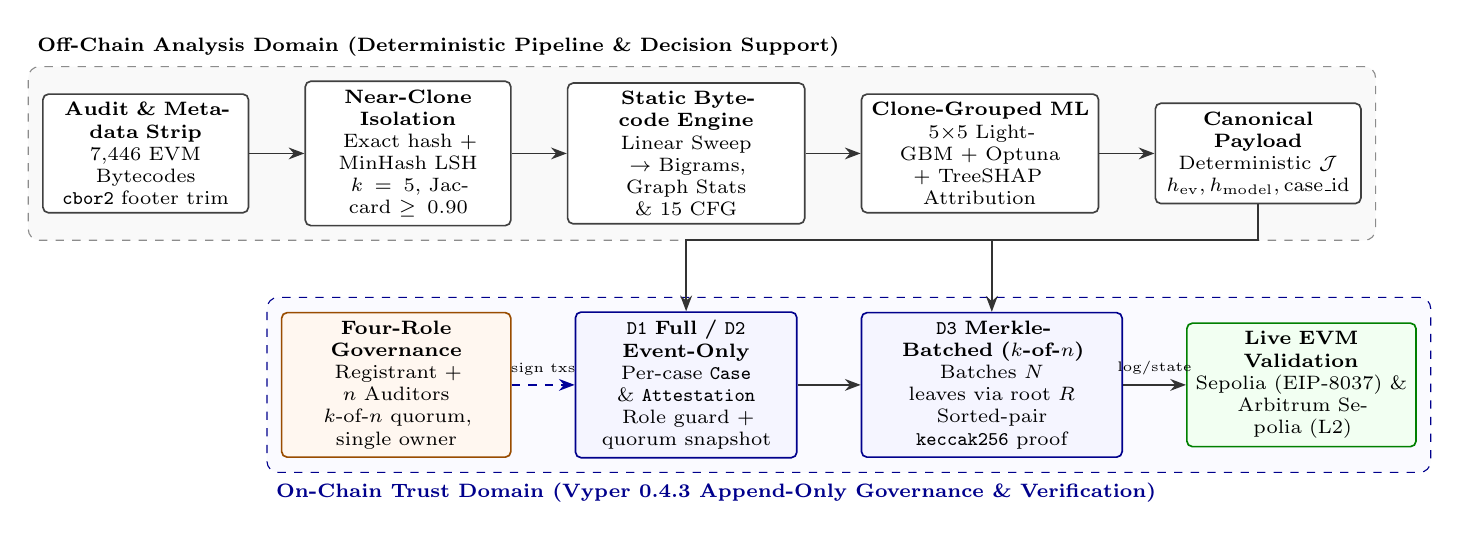
\begin{tikzpicture}[
    node distance=5mm and 7mm,
    font=\scriptsize,
    box/.style={draw=black!75, rounded corners=2pt, fill=white, align=center, minimum height=9mm, text width=24mm, inner sep=3pt, line width=0.6pt},
    widebox/.style={draw=black!75, rounded corners=2pt, fill=white, align=center, minimum height=9mm, text width=28mm, inner sep=3pt, line width=0.6pt},
    store/.style={draw=blue!55!black, rounded corners=2pt, fill=blue!4, align=center, minimum height=8.5mm, text width=26mm, inner sep=3pt, line width=0.6pt},
    arr/.style={-{Stealth[length=2mm]}, line width=0.65pt, draw=black!80},
    darr/.style={-{Stealth[length=2mm]}, line width=0.65pt, dashed, draw=blue!60!black}
]
% Row 1: Off-chain Data & Feature Pipeline
\node[box] (corpus) {\textbf{Audit \& Metadata Strip}\\7,446 EVM Bytecodes\\\texttt{cbor2} footer trim};
\node[box, right=of corpus] (lsh) {\textbf{Near-Clone Isolation}\\Exact hash + MinHash LSH\\$k=5$, Jaccard $\ge 0.90$};
\node[widebox, right=of lsh] (feats) {\textbf{Static Bytecode Engine}\\Linear Sweep $\to$ Bigrams,\\Graph Stats \& 15 CFG};
\node[widebox, right=of feats] (ml) {\textbf{Clone-Grouped ML}\\5$\times$5 LightGBM + Optuna\\+ TreeSHAP Attribution};
\node[box, right=of ml] (json) {\textbf{Canonical Payload}\\Deterministic $\mathcal{J}$\\$h_{\text{ev}}, h_{\text{model}}, \text{case\_id}$};

% Row 2: On-chain Vyper Registries & Verification
\node[store, below=11mm of feats] (d12) {\textbf{\texttt{D1} Full / \texttt{D2} Event-Only}\\Per-case \texttt{Case} \& \texttt{Attestation}\\Role guard + quorum snapshot};
\node[store, right=8mm of d12, text width=31mm] (d3) {\textbf{\texttt{D3} Merkle-Batched ($k$-of-$n$)}\\Batches $N$ leaves via root $R$\\Sorted-pair \texttt{keccak256} proof};
\node[box, right=8mm of d3, text width=27mm, fill=green!5, draw=green!50!black] (chains) {\textbf{Live EVM Validation}\\Sepolia (EIP-8037) \&\\Arbitrum Sepolia (L2)};
\node[box, left=8mm of d12, text width=27mm, fill=orange!6, draw=orange!60!black] (auditors) {\textbf{Four-Role Governance}\\Registrant + $n$ Auditors\\$k$-of-$n$ quorum, single owner};

% Background Trust Boundary Frames (labels placed on outer edges to avoid arrow overlap)
\begin{scope}[on background layer]
\node[draw=black!45, dashed, rounded corners=4pt, fill=gray!5, fit=(corpus)(lsh)(feats)(ml)(json), inner sep=5pt, label={[font=\scriptsize\bfseries, anchor=south west]north west:{Off-Chain Analysis Domain (Deterministic Pipeline \& Decision Support)}}] (bg_off) {};
\node[draw=blue!55!black, dashed, rounded corners=4pt, fill=blue!2, fit=(auditors)(d12)(d3)(chains), inner sep=5pt, label={[font=\scriptsize\bfseries, text=blue!55!black, anchor=north west]south west:{On-Chain Trust Domain (Vyper 0.4.3 Append-Only Governance \& Verification)}}] (bg_on) {};
\end{scope}

\draw[arr] (corpus) -- (lsh);
\draw[arr] (lsh) -- (feats);
\draw[arr] (feats) -- (ml);
\draw[arr] (ml) -- (json);
\draw[arr] (json.south) -- ++(0,-4.5mm) -| (d12.north);
\draw[arr] (json.south) -- ++(0,-4.5mm) -| (d3.north);
\draw[darr] (auditors) -- node[above, font=\tiny]{sign txs} (d12);
\draw[arr] (d12) -- (d3);
\draw[arr] (d3) -- node[above, font=\tiny]{log/state} (chains);
\end{tikzpicture}
\caption{End-to-end X-SPIDE-G architecture separating off-chain clone-isolated classification from immutable on-chain Vyper quorum governance\@.}
\label{fig:architecture}
\end{figure*}

X-SPIDE-G isolates probabilistic off-chain risk scoring from deterministic on-chain attestation governance (Fig.~\ref{fig:architecture}). Model scores and SHAP drivers act strictly as auditable decision-support artifacts rather than autonomous enforcement mechanisms.

\subsection{Trust Boundaries, Role Separation, and Security Invariants}\label{sec:roles}

On-chain governance enforces strict separation among four distinct participant roles:
\begin{enumerate}
\item \emph{Governance Owner:} Registers or removes auditor addresses and configures quorum threshold $k \ge 1$. Contract guards prohibit self-assignment as an auditor and reject thresholds exceeding active auditor counts.
\item \emph{Accredited Auditors ($n$ addresses):} Independently submit \texttt{Approve}, \texttt{Reject}, or \texttt{NeedsReview} verdicts via client-side wallet signatures. Each auditor can revise a vote monotonically while preserving revision history.
\item \emph{Case Registrant:} Anchors deterministic off-chain classification metadata into the registry. In our implementation, any accredited auditor may initiate a case, preventing unauthenticated state spam.
\item \emph{Public Verifier:} Queries contract state or calls read-only verification functions off-chain to confirm evidence integrity at zero transaction fee.
\end{enumerate}

\begin{table}[t]
\centering
\caption{Trust Comparison: Mutable Signed Database vs.\ On-Chain Registry}
\label{tab:threat_summary}
\footnotesize
\setlength{\tabcolsep}{3pt}
\begin{tabular}{@{}llll@{}}
\toprule
Threat Scenario & Signed Database & $k$-of-$n$ Registry & Suite \\
\midrule
Score/SHAP edit & Overwritable & Fixed \texttt{evidence\_hash} & \texttt{T2, T8} \\
Vote repudiation & Sig.\ logged & Wallet \texttt{Attested} rev. & \texttt{T5, T9} \\
Admin deletion & Truncatable & Append-only API & \texttt{T6, T7} \\
1-key collusion & 1 key suffices & $\ge k$ distinct votes & \texttt{T4, T10} \\
Open-case Sybil/$k$ & Mutable rule & Snapshot $k$ + nonce & \texttt{T13} \\
Server key leak & Key exposed & Client wallet sign & Audit \\
Replay attack & Weak ID join & ABI \texttt{chain\_id} hash & Unit \\
\bottomrule
\end{tabular}
\end{table}

Table~\ref{tab:threat_summary} contrasts our $k$-of-$n$ Vyper registry against a conventional database storing signed records, using Application Binary Interface (ABI) domain binding for cross-chain replay defense. Across automated verification tests \texttt{T1}--\texttt{T13} (46 contract tests), all three Vyper variants achieve 100\% explicit \texttt{assert} branch coverage (\texttt{D1} 20/20, \texttt{D2} 20/20, \texttt{D3} 18/18) and enforce seven security invariants:
\begin{itemize}
\item \emph{Access Rejection (\texttt{T1}, \texttt{T6}):} Non-auditors and the owner revert when invoking registration or attestation calls.
\item \emph{Evidence Binding (\texttt{T2}, \texttt{T8}):} Duplicate \texttt{case\_id} entries and zero digests revert, and hash-tampered payloads fail verification.
\item \emph{Quorum Determinism (\texttt{T3}, \texttt{T4}, \texttt{T11}):} Status recomputation evaluates consensus across all 27 three-auditor vote combinations for $k=2$ of $n=3$.
\item \emph{Vote Versioning (\texttt{T5}, \texttt{T9}):} Vote updates increment a strict per-auditor revision counter and emit prior decision logs.
\item \emph{Append-Only Persistence (\texttt{T6}, \texttt{T7}):} Interfaces expose zero deletion or overwrite methods and reject stray Ether transfers.
\item \emph{Merkle Integrity (\texttt{T12}):} Inclusion proofs check sorted-pair \texttt{keccak256} paths, rejecting single-bit leaf or proof corruptions.
\item \emph{Quorum Isolation \& Revocation (\texttt{T13}):} Registration snapshots \texttt{required\_\allowbreak threshold} and \texttt{created\_\allowbreak roster\_\allowbreak nonce}, blocking post-creation auditors, routing ties ($\text{approve}\ge k \land \text{reject}\ge k$) symmetrically to \texttt{Disputed}, and allowing vote cleanup for removed auditors strictly on open records while locking finalized verdicts.
\end{itemize}

While \texttt{T13} enforces threshold snapshotting, Sybil roster isolation, tie-safe \texttt{Disputed} resolution, and open-case vote cleanup directly in bytecode for all existing records, this prototype retains a single externally owned account (EOA) deployer key as governance owner for \emph{future} roster and threshold updates; production deployments must migrate ownership to a multisignature timelock. Off-chain model integrity additionally remains a distinct upstream trust assumption authenticated only via its anchored Secure Hash Algorithm 256-bit (SHA-256) weight digest.

\subsection{Corpus Audit, Metadata Stripping, and Clone Clustering}\label{sec:corpus}

We audit the official X-SPIDE release~\cite{pennella2025repo}, confirming 7,446 labeled contracts ($880$ Ponzi, $6{,}566$ non-Ponzi, zero label conflicts) across 23 account and 76 opcode baseline columns. Live remote procedure call (RPC) checks confirm 100.0\% active bytecode availability across all 880 Ponzi contracts and 880 sampled non-Ponzi contracts.

Comparing the 7,446 retained records against the pre-filtered 7,962-contract archive exposes 516 excluded entries (54 Ponzi, 462 non-Ponzi). Kolmogorov--Smirnov (KS) tests reveal significant selection bias toward shorter-lived excluded contracts with higher outgoing activity (\texttt{tx\_out} KS $=0.2467$, $p=2.50\times 10^{-26}$). Median lifetime drops from 15 to 2 days among excluded contracts (KS $=0.1384$, $p=1.58\times 10^{-8}$), where 308 missing-bytecode entries return empty code (\texttt{0x}) live. Throughout this study, $S_{\text{code}}$ denotes the verified 7,446-contract corpus with recovered runtime bytecode.

Solidity ($\ge$ v0.4.7) and Vyper compilers append a Concise Binary Object Representation (CBOR) metadata trailer terminating deployed code~\cite{soliditymetadata}. Parsing the trailing 2-byte big-endian footer length and decoding payloads via \texttt{cbor2} against known keys (\texttt{solc}, \texttt{vyper}, \texttt{ipfs}, \texttt{bzzr0}, \texttt{bzzr1}) strips trailers across 6,417 contracts, leaving 1,029 legacy or hand-written bytecodes untouched. Cross-referencing external benchmarks finds 161/182 Unica addresses~\cite{unica2021ponzi} and 122/139 PonziGuard contracts~\cite{liang2024repo} already inside X-SPIDE\@. Removing overlaps yields 107 disjoint external binaries (10 unique Ponzi hashes over 11 rows, 97 non-Ponzi) used as an external directional sanity screen (\texttt{E6}).

We construct two deterministic clone partitionings over $S_{\text{code}}$:
\begin{enumerate}
\item \emph{Exact Clusters (\texttt{group\_exact}):} Groups contracts by \texttt{keccak256} over CBOR-stripped bytecode, creating 6,145 clusters (5,696 singletons, max size 91, 10 mixed-label clusters) placing 225/880 (25.57\%) Ponzi instances in multi-contract groups.
\item \emph{Near-Clone Clusters (\texttt{group\_near}):} Extracts 5-gram normalized opcode shingles~\cite{broder1997resemblance}, indexes 128-permutation MinHash LSH signatures at threshold 0.90, and verifies exact candidate Jaccard similarity $\ge 0.90$. Connected components yield 4,711 clusters (3,825 singletons, max size 99, 24 mixed-label clusters) uniting 520/880 (59.09\%) Ponzi contracts and 3,101/6,566 (47.23\%) non-Ponzi contracts in shared families.
\end{enumerate}

\section{Methodology and Governance Architecture}\label{sec:method}

Building upon the verified corpus $S_{\text{code}}$ and near-clone groupings, this section details our static feature extractors, nested evaluation protocol, and Vyper storage designs.

\subsection{Disassembly and Bytecode Feature Families}\label{sec:features}

Our deterministic linear-sweep disassembler parses EVM bytecode up to Cancun~\cite{wood2014ethereum}, handling EIP-3855 \texttt{PUSH0} (\texttt{0x5F}), logging truncated \texttt{PUSH} immediates on 554 contracts, and marking unassigned bytes as \texttt{INVALID\_XX} on 1,163 contracts with zero failures. Instruction normalization preserves \texttt{PUSH0} and collapses parameterized opcodes (\texttt{PUSH1}--\texttt{PUSH32}, \texttt{DUP1}--\texttt{DUP16}, \texttt{SWAP1}--\texttt{SWAP16}, \texttt{LOG0}--\texttt{LOG4}) into family tokens (\texttt{PUSH}, \texttt{DUP}, \texttt{SWAP}, \texttt{LOG}). Measured on an Intel Core i5-12450H CPU (12 logical threads, 15.63~GB RAM, Python 3.12.13), end-to-end extraction requires 13.885~ms median latency per contract (Table~\ref{tab:extraction_cost}), scaling in $O(L)$ time over $L$ bytecode instructions for disassembly and bigram indexing and $O(|V_C| + |E_C|)$ time for Tarjan SCC traversal. Three static representations are extracted:

\begin{table}[t]
\centering
\caption{Bytecode Feature Extraction Cost Across 7,446 Contracts}
\label{tab:extraction_cost}
\footnotesize
\setlength{\tabcolsep}{4pt}
\begin{tabular}{@{}lrrrr@{}}
\toprule
Pipeline Stage & Dim & Median (ms) & p95 (ms) & Errors \\
\midrule
Disassembly & -- & 3.305 & 11.999 & 0 \\
F-BIGRAM & 200 & 3.073 & 9.224 & 0 \\
F-GSTAT & 16 & 1.618 & 4.761 & 0 \\
F-GSEM & 15 & 5.587 & 15.984 & 0 \\
End-to-End Runtime & 231 & 13.885 & 50.839 & 0 \\
\bottomrule
\end{tabular}
\end{table}

\begin{table}[t]
\centering
\caption{Summary of the 15 CFG-Semantic Descriptors (\texttt{F-GSEM})}
\label{tab:gsem_features}
\scriptsize
\setlength{\tabcolsep}{2.5pt}
\begin{tabular}{@{}l>{\raggedright\arraybackslash}p{3.45cm}>{\raggedright\arraybackslash}p{3.45cm}@{}}
\toprule
Group & Feature Name(s) & Structural Definition \\
\midrule
CFG \& & \texttt{n\_blocks}, \texttt{n\_cfg\_edges} & Block count $|V_C|$ and edges $|E_C|$ \\
Jumps & \texttt{cyclomatic}, \texttt{unresolved\_jump\_ratio} & $M_C$ \eqref{eq:cfg_cyclomatic} and indirect share \eqref{eq:unresolved_ratio} \\
\midrule
SCC & \texttt{n\_scc\_cycles}, \texttt{n\_loops\_with\_sstore} & Non-trivial SCCs and store loops \\
Loops & \texttt{n\_loops\_with\_call}, \texttt{has\_loop\_with\_call} & \texttt{CALL}-bearing SCC count and flag \\
 \& Call & \texttt{n\_blocks\_with\_call}, \texttt{call\_block\_ratio} & \texttt{CALL} blocks and $|V_{\text{CALL}}|/|V_C|$ \\
\midrule
Flow \& & \texttt{path\_callvalue\_to\_call} & Path from \texttt{CALLVALUE} to \texttt{CALL} \\
Centr. & \texttt{pagerank\_CALL}, \texttt{pagerank\_SSTORE} & Transition-graph PageRank \\
 & \texttt{has\_selfdestruct}, \texttt{selfdestruct\_reachable} & \texttt{SELFDESTRUCT} flag and reachability \\
\bottomrule
\end{tabular}
\end{table}

\begin{itemize}
\item \emph{Normalized Opcode Bigrams (\texttt{F-BIGRAM}):} Relative frequencies over adjacent normalized opcode pairs. Each fold selects the top 200 bigrams exclusively from its training partition.
\item \emph{Transition-Graph Statistics (\texttt{F-GSTAT}):} Sixteen scalar summaries constructed from normalized opcode adjacency graphs, tracking vertex and edge counts, total transitions, mean and maximum weighted in/out degrees, transition Shannon entropy, self-loop ratios, density ($|E|/|V|^2$), and instruction-length ($/L$) normalized variants.
\item \emph{CFG and Loop Semantics (\texttt{F-GSEM}):} Basic blocks terminate at \texttt{JUMP}, \texttt{JUMPI}, \texttt{STOP}, \texttt{RETURN}, \texttt{REVERT}, \texttt{INVALID}, or \texttt{SELFDESTRUCT}. Static jump resolution tracks immediate \texttt{PUSH} offsets directly preceding jumps, extracting the 15 features in Table~\ref{tab:gsem_features}.
\end{itemize}

For each control-flow graph, multi-component McCabe cyclomatic complexity follows~\eqref{eq:cfg_cyclomatic},
\begin{equation}\label{eq:cfg_cyclomatic}
M_C = |E_C| - |V_C| + 2P,
\end{equation}
where $|E_C|$ and $|V_C|$ denote directed CFG edges and basic blocks, and $P \ge 1$ counts weakly connected components. Accounting for $P$ guarantees $M_C \ge P \ge 1$ across all 7,446 contracts (min $1$, median $40$, max $547$; zero negative values even when indirect jumps fragment blocks across multiple components). We measure jump ambiguity via~\eqref{eq:unresolved_ratio}:
\begin{equation}\label{eq:unresolved_ratio}
r_{\text{unres}} = \frac{J_{\text{unres}}}{J_{\text{total}}},
\end{equation}
where $J_{\text{unres}}$ counts indirect jump sites lacking a preceding immediate target among $J_{\text{total}}$ total jumps. Across $S_{\text{code}}$, median $r_{\text{unres}}$ is $0.1918$ (mean $0.2498$), with $526/7{,}446$ contracts ($7.06\%$) exceeding $0.50$.

\subsection{Nested Evaluation and Dual Statistical Protocol}\label{sec:stats}

Primary clone-grouped models (\texttt{E1}--\texttt{E4d}) share identical $5 \times 5$ repeated \texttt{StratifiedGroupKFold} splits~\cite{pedregosa2011scikit} grouped on \texttt{group\_near} across seeds $\{42, \dots, 46\}$ (25 folds, $\approx 5{,}957$ train and $\approx 1{,}489$ test contracts). Within each outer fold, inner 3-fold \texttt{StratifiedGroupKFold} runs 30 Optuna Tree-structured Parzen Estimator (TPE) trials~\cite{akiba2019optuna} tuning LightGBM~\cite{ke2017lightgbm} depth, leaves, subsampling, regularization, and imbalance weighting to maximize PR-AUC\@. Decision thresholds $\tau^*$ maximize inner Out-of-Fold (OOF) F1, while \texttt{E2} additionally executes in-fold recursive feature elimination (RFECV).

For paired fold metric differences $d_1, \dots, d_{25}$ ($n_{\text{test}}/n_{\text{train}} \approx 0.25$), we apply the Nadeau--Bengio (NB) variance-corrected $t$-test ($df=24$) in~\eqref{eq:nadeau_bengio}~\cite{nadeau2003inference}:
\begin{equation}\label{eq:nadeau_bengio}
t_{\text{NB}} = \frac{\bar{d}}{\sqrt{\left(\frac{1}{25} + \frac{0.25}{1}\right) s_d^2}},
\end{equation}
where $\bar{d}$ and $s_d^2$ denote sample mean and Bessel-corrected variance across the 25 outer differences. To reconcile parametric confidence intervals (CIs) with our pre-registered test suite, we report both Holm--Bonferroni adjusted parametric values ($p_{\text{Holm,NB}}$) and pre-registered Wilcoxon signed-rank Holm adjustments ($p_{\text{Holm,W}}$) over all eight primary tests~\cite{holm1979simple}. A gain is confirmed only when meeting three criteria: $\Delta\text{PR-AUC} \ge 0.0200$ (minimum detectable effect, MDE), 95\% NB CI strictly above zero, and $p_{\text{Holm,NB}} < 0.05$.

\subsection{Canonical Evidence Binding and Vyper Variants}\label{sec:variants}

Once off-chain inference produces score $p$, threshold $\tau^*$, and top-$K$ TreeSHAP values~\cite{lundberg2017shap}, X-SPIDE-G serializes a canonical JavaScript Object Notation (JSON) artifact $\mathcal{J}$ (sorted keys, fixed 6-decimal strings) hashed via $h_{\text{ev}} = \texttt{evidence\_hash} = \operatorname{keccak256}(\mathcal{J})$. Weight reproducibility is pinned by $h_{\text{model}} = \texttt{model\_version\_hash}$. Contracts bind cross-chain identifiers deterministically via~\eqref{eq:case_id}:
\begin{equation}\label{eq:case_id}
\begin{aligned}
\text{case\_id} = \operatorname{keccak256}\bigl(&\operatorname{abi\_encode}(\text{chain\_id},\\
&\text{subject}, h_{\text{model}}, \text{run\_id})\bigr),
\end{aligned}
\end{equation}
where $\operatorname{abi\_encode}$ packs the EIP-155 network identifier, audited contract \texttt{subject}, weight digest $h_{\text{model}}$, and 32-byte execution nonce $\text{run\_id}$ (while public verification cross-checks $h_{\text{ev}}$, \texttt{subject}, \texttt{chain\_id}, $h_{\text{model}}$, and \texttt{case\_id} against on-chain \texttt{Case} records).

We implement and compare three Vyper 0.4.3 (\texttt{\string^0.4.0}) registry designs:
\begin{itemize}
\item \emph{\texttt{D1} (Full-Storage Registry):} Persists complete \texttt{Case} and per-auditor \texttt{Attestation} structs in contract storage for direct smart-contract lookup.
\item \emph{\texttt{D2} (Event-Only Registry):} Compresses storage to vote counts, status, and \texttt{evidence\_hash}, offloading strings and reasons to indexed logs.
\item \emph{\texttt{D3} (Merkle-Batched Registry):} Anchors $N$ off-chain leaves, each hashing the ABI-encoded tuple $(\text{case\_id}, h_{\text{ev}}, h_{\text{model}})$ via \texttt{keccak256}, under one root in $O(1)$ on-chain write gas, verified via $O(\log_2 N)$ sorted-pair proofs. Because \texttt{D3} records one quorum status per root, heterogeneous verdicts must be partitioned into verdict-homogeneous sub-batches before anchoring.
\end{itemize}

\section{Experimental Evaluation}\label{sec:eval}

Our empirical study evaluates paper-style baseline reproduction and clone leakage (\texttt{E0}--\texttt{E1}), controlled feature-family ablations (\texttt{E1}--\texttt{E4d}), preprocessing sensitivities (\texttt{S0}--\texttt{S4}, \texttt{E6}), and multi-chain Vyper attestation benchmarks (\texttt{E5}, \texttt{T1}--\texttt{T13}). We report PR-AUC, F1, ROC-AUC, and high-precision recall at $\ge 0.90$ precision (R@P0.9). All model ablations shared identical 25-fold near-clone-grouped splits unless explicitly testing exact or random partitioning.

\subsection{RQ1: Baseline Reproduction and Clone-Leakage Quantification}\label{sec:rq1}

\begin{table}[t]
\centering
\caption{RQ1: Baseline Reproduction and Clone-Leakage Impact (LightGBM)}
\label{tab:rq1_leakage}
\scriptsize
\setlength{\tabcolsep}{2.5pt}
\begin{tabular}{@{}llrrrrr@{}}
\toprule
Experiment & Split Protocol & Feats & PR-AUC & F1 & ROC-AUC & R@P0.9 \\
\midrule
Published~\cite{pennella2025xspide} & 85/15 random & 47 & -- & 0.8670 & 0.9770 & -- \\
\texttt{E0} (47 unbal.) & 85/15 random & 47 & 0.9173 & 0.8340 & 0.9772 & 0.8030 \\
\texttt{E0} (99 CV) & Random 5-fold & 99 & 0.9149 & 0.8589 & 0.9768 & 0.8273 \\
\midrule
\texttt{E1-S0} (ctrl) & \texttt{random} 5$\times$5 & 99 & 0.9251 & 0.8679 & 0.9785 & 0.8393 \\
\texttt{E1-Exact} & \texttt{group\_exact} 5$\times$5 & 99 & 0.9051 & 0.8379 & 0.9730 & 0.7895 \\
\texttt{E1} (X-SPIDE) & \texttt{group\_near} 5$\times$5 & 99 & 0.8767 & 0.8118 & 0.9631 & 0.7141 \\
\bottomrule
\end{tabular}
\end{table}

Table~\ref{tab:rq1_leakage} confirms reproduction fidelity while isolating split leakage from tuning-protocol shifts via a controlled three-step causal decomposition. Re-running the published 47-feature pipeline (\texttt{E0}) matched ROC-AUC within $+0.0002$ ($0.9772$ vs.\ $0.9770$), with F1 differing slightly ($0.8340$ vs.\ $0.8670$) due to library version evolution and unarchived thresholding~\cite{pennella2025repo}. Upgrading the 99-feature random setup from paper-style 5-fold grid search (\texttt{E0}: $0.9149$ PR-AUC, fixed $0.5$ cutoff) to $5\times 5$ nested Optuna with inner OOF thresholding (\texttt{E1-S0}: $0.9251$ PR-AUC, $0.8679$ F1) raised PR-AUC by $+0.0102$ ($+0.0090$ F1) purely from tuning protocol. Holding that identical $5\times 5$ nested protocol strictly fixed, exact deduplication (\texttt{E1-S0} $\to$ \texttt{E1-Exact}: $0.9051$) removed $-0.0201$ PR-AUC ($-0.0300$ F1) of pure exact-clone leakage, and MinHash near-clone quarantine (\texttt{E1-Exact} $\to$ \texttt{E1}: $0.8767$) removed another $-0.0283$ PR-AUC ($-0.0261$ F1). Total pure clone leakage therefore reached $-0.0484$ PR-AUC, $-0.0561$ F1, and $-0.1252$ R@P0.9, demonstrating that the net \texttt{E0} $\to$ \texttt{E1} drop ($-0.0382$ PR-AUC) actually underestimated true clone leakage.

\subsection{RQ2: Bytecode Ablations and Statistical Significance}\label{sec:rq2}

\begin{table*}[t]
\centering
\caption{RQ2: Feature-Family Ablation Under Clone-Grouped $5 \times 5$ Nested Cross-Validation (25 Outer Folds)}
\label{tab:rq2_ablation}
\footnotesize
\setlength{\tabcolsep}{5pt}
\begin{tabular}{@{}llrrrrrrr@{}}
\toprule
Exp & Feature Representation & Feats & PR-AUC (mean $\pm$ std) & $\Delta$PR-AUC vs.\ E1 & F1 (mean $\pm$ std) & ROC-AUC & R@P0.9 \\
\midrule
\texttt{E1} & 99 X-SPIDE baseline & 99 & $0.8767 \pm 0.0254$ & $0.0000$ & $0.8118 \pm 0.0275$ & 0.9631 & 0.7141 \\
\texttt{E2} & In-fold RFECV over 99 & 71.4 & $0.8768 \pm 0.0237$ & $+0.0000$ & $0.8095 \pm 0.0264$ & 0.9638 & 0.7148 \\
\texttt{E3} & \texttt{F-GSTAT} only & 16 & $0.6000 \pm 0.0629$ & $-0.2767$ & $0.5364 \pm 0.0703$ & 0.8402 & 0.2711 \\
\texttt{E3b} & \texttt{F-BIGRAM} only (top-200) & 200 & $\mathbf{0.9013} \pm 0.0191$ & $+0.0246$ & $0.8247 \pm 0.0241$ & 0.9736 & 0.7520 \\
\texttt{E3c} & \texttt{F-GSEM} only & 15 & $0.7832 \pm 0.0421$ & $-0.0935$ & $0.7049 \pm 0.0395$ & 0.9269 & 0.5077 \\
\texttt{E4} & 99 X-SPIDE + \texttt{F-GSTAT} & 115 & $0.8805 \pm 0.0242$ & $+0.0037$ & $0.8140 \pm 0.0243$ & 0.9641 & 0.7241 \\
\texttt{E4b} & 99 X-SPIDE + \texttt{F-BIGRAM} & 299 & $0.8995 \pm 0.0212$ & $+0.0227$ & $0.8263 \pm 0.0269$ & $\mathbf{0.9738}$ & 0.7548 \\
\texttt{E4c} & 99 X-SPIDE + \texttt{F-GSEM} & 114 & $0.8842 \pm 0.0237$ & $+0.0075$ & $0.8144 \pm 0.0295$ & 0.9657 & 0.7370 \\
\texttt{E4d} & 99 X-SPIDE + \texttt{F-BIGRAM} + \texttt{F-GSEM} & 314 & $0.9011 \pm 0.0191$ & $+0.0244$ & $\mathbf{0.8267} \pm 0.0241$ & $\mathbf{0.9738}$ & $\mathbf{0.7677}$ \\
\bottomrule
\end{tabular}
\end{table*}

\begin{table*}[t]
\centering
\caption{Pre-Registered Eight-Comparison Statistical Tests ($\Delta$PR-AUC, Nadeau--Bengio $\rho=0.25$ vs.\ Wilcoxon Holm)}
\label{tab:stat_tests}
\scriptsize
\setlength{\tabcolsep}{3.5pt}
\begin{tabular}{@{}lrrrrrl@{}}
\toprule
Pairwise Comparison & $\Delta$PR-AUC & 95\% Nadeau--Bengio CI & $p_{\text{NB}}$ & $p_{\text{Holm,NB}}$ & $p_{\text{Holm,W}}$ & Combined Verdict \\
\midrule
\texttt{E4b} vs.\ \texttt{E1} (+\texttt{F-BIGRAM} over base) & $+0.0227$ & $[+0.0096, +0.0358]$ & $1.55\times 10^{-3}$ & $9.27\times 10^{-3}$ & $4.77\times 10^{-7}$ & Confirmed Gain \\
\texttt{E3c} vs.\ \texttt{E3} (\texttt{F-GSEM} vs.\ \texttt{F-GSTAT}) & $+0.1832$ & $[+0.1271, +0.2394]$ & $5.78\times 10^{-7}$ & $4.04\times 10^{-6}$ & $4.77\times 10^{-7}$ & Confirmed Gain \\
\texttt{E4} vs.\ \texttt{E1} (+\texttt{F-GSTAT} over base) & $+0.0037$ & $[-0.0027, +0.0102]$ & $0.2457$ & $0.7370$ & $0.0138$ & No Sig.\ Diff.\ (CI spans 0) \\
\texttt{E4c} vs.\ \texttt{E1} (+\texttt{F-GSEM} over base) & $+0.0075$ & $[-0.0029, +0.0179]$ & $0.1509$ & $0.6036$ & $2.53\times 10^{-3}$ & No Sig.\ Diff.\ (CI spans 0) \\
\texttt{E4d} vs.\ \texttt{E4b} (+\texttt{F-GSEM} atop \texttt{F-BIGRAM}) & $+0.0017$ & $[-0.0091, +0.0125]$ & $0.7504$ & $1.0000$ & $0.5992$ & No Sig.\ Diff.\ \\
\texttt{E2} vs.\ \texttt{E1} (In-fold RFECV vs.\ all 99) & $+0.0000$ & $[-0.0070, +0.0071]$ & $0.9929$ & $1.0000$ & $1.0000$ & No Sig.\ Diff.\ \\
\texttt{E4c} vs.\ \texttt{E4b} (\texttt{F-GSEM} vs.\ \texttt{F-BIGRAM}) & $-0.0152$ & $[-0.0275, -0.0030]$ & $0.0171$ & $0.0853$ & $9.83\times 10^{-6}$ & Neg.\ CI ($p_{\text{Holm,NB}}>0.05$) \\
\texttt{E3c} vs.\ \texttt{E3b} (\texttt{F-GSEM} vs.\ \texttt{F-BIGRAM} only) & $-0.1181$ & $[-0.1524, -0.0838]$ & $2.41\times 10^{-7}$ & $1.93\times 10^{-6}$ & $4.77\times 10^{-7}$ & Significant Drop \\
\bottomrule
\end{tabular}
\end{table*}

\begin{figure}[t]
\centering
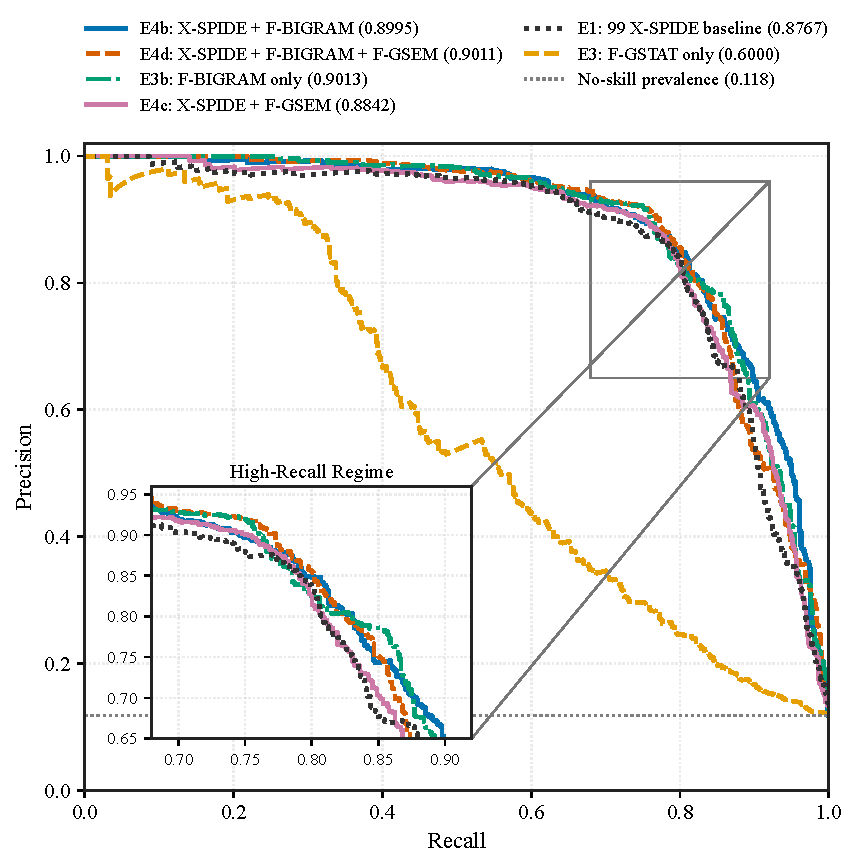
\includegraphics[width=\columnwidth]{figures/pr_curves.pdf}
\caption{Pooled out-of-fold Precision--Recall curves (seed 42) across key feature configurations, with an inset magnifying high-recall separation. Legend values report 25-fold outer CV means.}
\label{fig:pr_curves}
\end{figure}

\begin{figure*}[t]
\centering
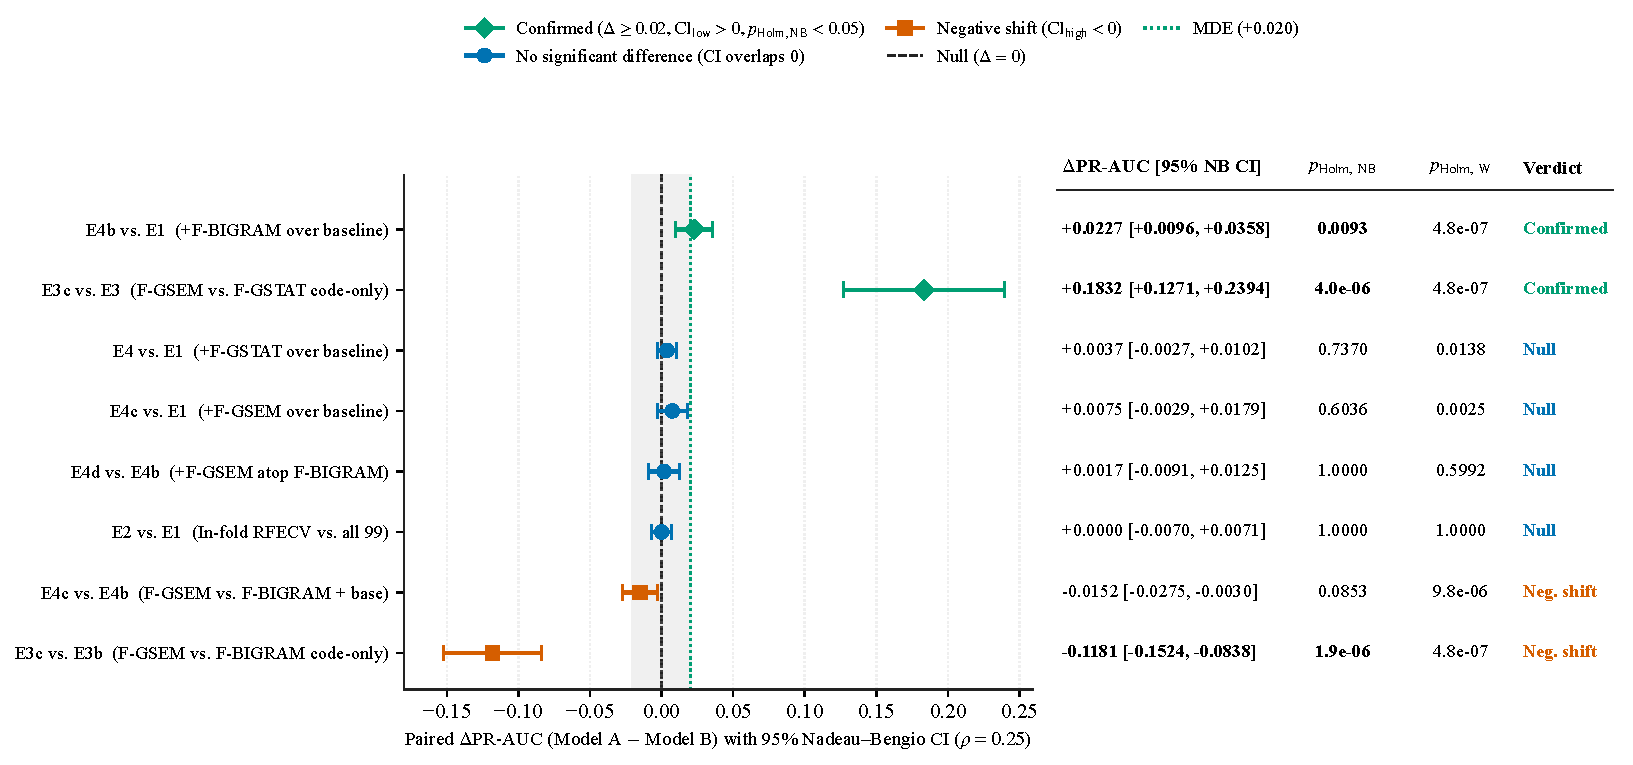
\includegraphics[width=\textwidth]{figures/delta_pr_auc_ci.pdf}
\caption{Forest plot of paired $\Delta$PR-AUC with 95\% Nadeau--Bengio confidence intervals ($\rho=0.25$) alongside both parametric ($p_{\text{Holm,NB}}$) and pre-registered Wilcoxon ($p_{\text{Holm,W}}$) Holm--Bonferroni values.}
\label{fig:forest_ci}
\end{figure*}

Tables~\ref{tab:rq2_ablation}--\ref{tab:stat_tests} and Figs.~\ref{fig:pr_curves}--\ref{fig:forest_ci} reveal a sharp architectural contrast among static bytecode representations:
\begin{enumerate}
\item \emph{Local Opcode Bigrams Excel:} Adding \texttt{F-BIGRAM} over the 99 X-SPIDE baseline (\texttt{E4b} vs.\ \texttt{E1}) elevated PR-AUC by $+0.0227$ to $0.8995$ (95\% NB CI $[+0.0096, +0.0358]$, $p_{\text{Holm,NB}}=0.0093$, $p_{\text{Holm,W}}=4.77\times 10^{-7}$), clearing the pre-registered MDE\@. Code-only \texttt{F-BIGRAM} (\texttt{E3b}) reached $0.9013$ PR-AUC without any transaction counts.
\item \emph{Semantic CFG Metrics vs.\ Raw Transition Statistics:} Standalone \texttt{F-GSEM} (\texttt{E3c}, $0.7832$ PR-AUC) outperformed \texttt{F-GSTAT} (\texttt{E3}, $0.6000$) by $+0.1832$ ($p_{\text{Holm,NB}}=4.04\times 10^{-6}$), confirming that explicit loop--call structures retain stronger fraud signal than coarse degree averages.
\item \emph{Marginal Utility Over Bigrams:} Adding \texttt{F-GSEM} over X-SPIDE (\texttt{E4c} vs.\ \texttt{E1}, $+0.0075$) crossed zero under the parametric NB interval ($p_{\text{Holm,NB}}=0.6036$), even though paired Wilcoxon ranks appeared small ($p_{\text{Holm,W}}=2.53\times 10^{-3}$). Adding \texttt{F-GSEM} atop \texttt{F-BIGRAM} (\texttt{E4d} vs.\ \texttt{E4b}, $+0.0017$, $p_{\text{Holm,NB}}=1.0$) nudged R@P0.9 slightly from $0.7548$ to $0.7677$ without improving overall PR-AUC\@. Conversely, \texttt{E3c} trailed \texttt{E3b} significantly ($\Delta=-0.1181$).
\end{enumerate}

\begin{table}[t]
\centering
\caption{Sensitivity Analyses (\texttt{S0}--\texttt{S4}) and External Sanity Check (\texttt{E6})}
\label{tab:sensitivity}
\scriptsize
\setlength{\tabcolsep}{2.5pt}
\begin{tabular}{@{}llrrl@{}}
\toprule
Study & Variant vs.\ Reference & PR-AUC & $\Delta$PR & Outcome \\
\midrule
\texttt{S0} & \texttt{E1} random 5$\times$5 vs.\ near & 0.9251 & $+0.0484$ & Pure clone leakage \\
\texttt{S1} & \texttt{E1} exact vs.\ near & 0.9051 & $+0.0283$ & Near-clone bias \\
\texttt{S1} & \texttt{E4c} exact vs.\ near & 0.9104 & $+0.0261$ & Near-clone bias \\
\texttt{S2} & \texttt{E1} CBOR-stripped & 0.8792 & $+0.0024$ & Negligible \\
\texttt{S2} & \texttt{E4c} \texttt{F-GSEM} raw & 0.8811 & $-0.0032$ & Negligible \\
\texttt{S2} & \texttt{E4c} all CBOR-stripped & 0.8851 & $+0.0009$ & Negligible \\
\texttt{S3} & Latest 20\% block holdout & -- & -- & Deferred (no block ID) \\
\texttt{S4} & \texttt{E4b} raw opcodes & 0.8969 & $-0.0025$ & Negligible \\
\texttt{S4} & \texttt{E4c} raw PageRank & 0.8843 & $+0.0000$ & Negligible \\
\midrule
\texttt{E6} & PonziGuard (10 pos.) & 0.6169 & -- & Directional screen \\
\bottomrule
\end{tabular}
\end{table}

Table~\ref{tab:sensitivity} isolates preprocessing sensitivities. Stripping CBOR trailers (\texttt{S2}, $|\Delta| \le 0.0032$) and retaining raw unnormalized opcodes (\texttt{S4}, $|\Delta| \le 0.0025$) produced negligible shifts. Conversely, ungrouped random splitting (\texttt{S0}, $+0.0484$) and exact-hash grouping (\texttt{S1}, $+0.026$--$0.028$) confirmed substantial clone-leakage inflation.

Prospective temporal holdout (\texttt{S3}) remained infeasible because the source comma-separated values (CSV) file omits creation block numbers without archival BigQuery queries. External screening on 107 non-overlapping PonziGuard binaries (\texttt{E6}, 10 unique Ponzi hashes over 11 rows, 97 non-Ponzi, 291 code features) achieved $0.6169$ PR-AUC (95\% bootstrap CI $[0.3497, 0.8784]$), $0.7804$ ROC-AUC, and $0.5882$ F1\@. We interpret \texttt{E6} strictly as an underpowered directional sanity check.

\subsection{Explainability and Error-Mode Characterization}\label{sec:xai}

\begin{figure*}[t]
\centering
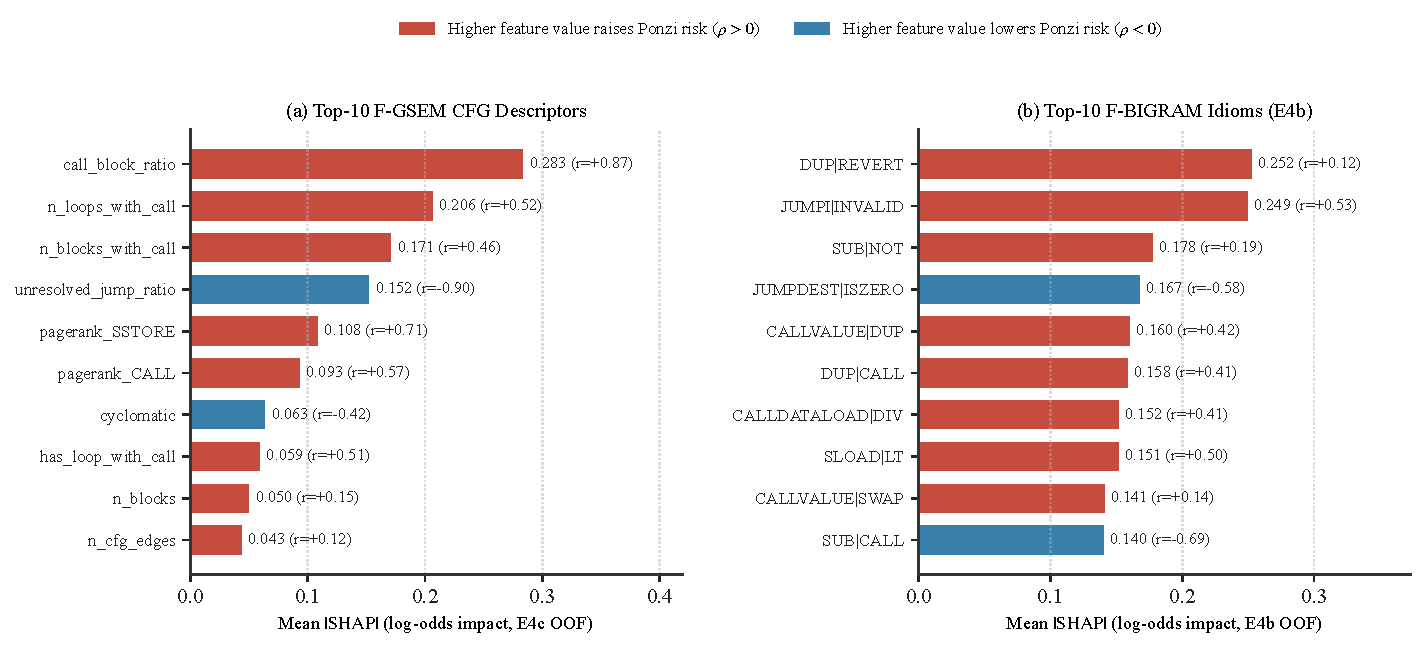
\includegraphics[width=\textwidth]{figures/shap_gsem_importance.pdf}
\caption{Global TreeSHAP feature importance (mean $|\text{SHAP}|$ in log-odds) and Spearman directionality ($\rho$) on seed-42 OOF predictions for (a) \texttt{F-GSEM} descriptors in \texttt{E4c} and (b) top \texttt{F-BIGRAM} idioms in \texttt{E4b}.}
\label{fig:shap}
\end{figure*}

Fig.~\ref{fig:shap}(a) shows that static CFG call density (\texttt{call\_\allowbreak block\_\allowbreak ratio}, mean $|\text{SHAP}|=0.2796$, $\rho=+0.848$) and SCC-enclosed calls (\texttt{n\_\allowbreak loops\_\allowbreak with\_\allowbreak call}, $0.2205$, conditional SHAP $+1.1058$ when positive vs.\ $-0.1239$ at zero) dominated \texttt{F-GSEM} attributions in \texttt{E4c}. High \texttt{unresolved\_\allowbreak jump\_\allowbreak ratio} ($0.1582$) inversely lowered log-odds ($\rho=-0.844$), reflecting complex routers with indirect dispatch.

Fig.~\ref{fig:shap}(b) illustrates why 200-feature \texttt{F-BIGRAM} outperformed 15-feature \texttt{F-GSEM} in \texttt{E4b}: whereas \texttt{F-GSEM} compresses the graph into coarse scalar counts, adjacent pairs retained fine-grained compiler failure guards (\texttt{DUP|REVERT} $0.2522$, \texttt{JUMPI|INVALID} $0.2494$, $\rho=+0.527$) and inflow-to-limit idioms (\texttt{CALLVALUE|DUP} $\rho=+0.418$, \texttt{SLOAD|LT} $\rho=+0.498$, \texttt{CALLDATALOAD|DIV} $\rho=+0.412$).

Auditing seed-42 \texttt{E4c} predictions---678 true positives (TP), 99 false positives (FP), 6,467 true negatives (TN), and 202 false negatives (FN)---exposed four failure mechanisms across 24 extreme-error reviews:
\begin{enumerate}
\item \emph{Benign Loops With \texttt{CALL} (3/12 audited FPs; plus 6/12 tx-asymmetry mimics):} Batch payout forwarders such as \texttt{0xdd39\ldots f347} ($p=0.9903$, $M_C=16$, one static \texttt{CALL} loop) confirmed that a \texttt{CALL} inside an SCC is a structural heuristic rather than proof of Ponzi redistribution.
\item \emph{Loop-Free Pull Ponzis (9/12 audited FNs):} Pull-withdrawal schemes like \texttt{0x4e18\ldots fd06} ($p=5.46\times 10^{-6}$, 0 static cycles) disburse funds per claim without an internal iteration loop.
\item \emph{CFG-Fragmented Proxies (1/12 audited FPs):} Dispatchers like \texttt{0x70e2\ldots 192a} ($p=0.9921$, $r_{\text{unres}}=0.5714$, 27 blocks, 26 edges, $P=4$, $M_C=7$) received negative \texttt{unresolved\_\allowbreak jump\_\allowbreak ratio} SHAP ($-0.330$), yet \texttt{SLOAD} ($+2.235$) and \texttt{AND} ($+1.344$) forced a false positive (larger routers like \texttt{0xf302\ldots 6538} reached $r_{\text{unres}}=0.9290$ with $544$ blocks, $301$ edges, $P=250$, and $M_C=257$).
\item \emph{Mixed-Label Clone Clusters:} Near-clone groups mixing benign and Ponzi labels accounted for 13/99 FPs and 38/202 FNs, reflecting up to 10\% opcode divergence within $J \ge 0.90$ clusters or dormant vs.\ active post-deployment behavior.
\end{enumerate}

\subsection{RQ3: On-Chain Cost, Latency, and Security Verification}\label{sec:rq3}

\begin{table*}[t]
\centering
\caption{RQ3: Gas and Anchored Cancun Cost in United States Dollars (USD) Across Simulation, Sepolia (EIP-8037), and Mainnet Regimes}
\label{tab:rq3_gas}
\scriptsize
\setlength{\tabcolsep}{3.5pt}
\begin{tabular}{@{}lrrrrrl@{}}
\toprule
Variant \& Operation & Cancun Sim. & Sepolia (EIP-8037) & Ref (0.9711 gwei) & Stress (30 gwei) & vs.\ D1 & Ceiling Check \\
\midrule
\texttt{D1} deploy (constructor) & 1,400,866 & 9,751,010 & \$2.3181 & \$71.61 & -- & Deployment \\
\texttt{D1} finalized case ($k=2$) & 484,818 & 1,881,226 & \$0.8022 & \$24.78 & -- & Fail ($>250\text{k}$) \\
\texttt{D1} \texttt{remove\_auditor} (warm) & 32,542 & 36,584 & \$0.0538 & \$1.66 & -- & Governance \\
\texttt{D1} \texttt{revoke\_removed\_auditor\_vote} & 46,864 & 63,402 & \$0.0775 & \$2.40 & -- & Open-case \texttt{T13} \\
\texttt{D2} EventOnly finalized ($k=2$) & 352,063 & 1,220,763 & \$0.5826 & \$18.00 & $-27.38\%$ & Fail ($>250\text{k}$) \\
\texttt{D3} MerkleBatch ($N=100$, /case) & 4,148.10 & 15,474.70 & \$0.0069 & \$0.21 & $-99.14\%$ & Pass ($\le 10\text{k}$ L2/Cancun) \\
\texttt{D3} MerkleBatch ($N=1000$, /case) & 414.82 & -- & \$0.0007 & \$0.02 & $-99.91\%$ & Pass ($\le 10\text{k}$) \\
\bottomrule
\end{tabular}
\end{table*}

\begin{figure}[t]
\centering
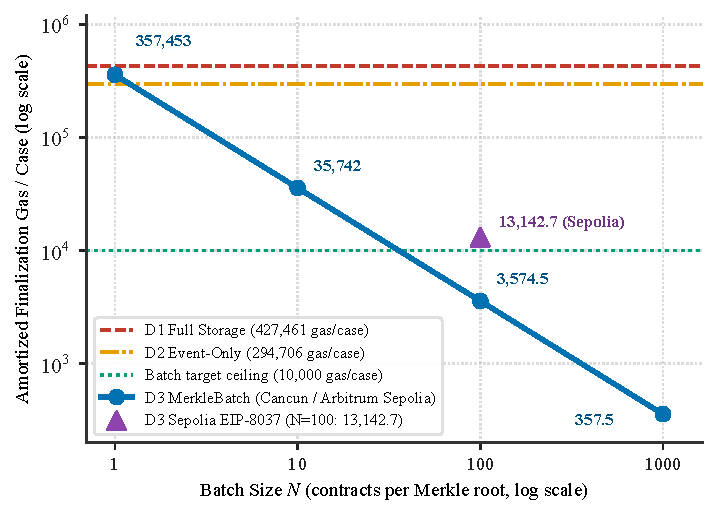
\includegraphics[width=\columnwidth]{figures/gas_vs_batch.pdf}
\caption{Amortized \texttt{D3} finalization gas per contract across batch sizes $N \in \{1, 10, 100, 1000\}$ under Cancun/L2 rules against single-case baselines (\texttt{D1}, \texttt{D2}) and measured Sepolia EIP-8037 points.}
\label{fig:gas}
\end{figure}

Table~\ref{tab:rq3_gas} and Fig.~\ref{fig:gas} quantify single-case vs.\ batched attestation scaling for our quorum-hardened registries. Full-storage \texttt{D1} required 484,818 Cancun gas ($k=2$ of $3$, adding $+57{,}357$ gas for \texttt{T13} threshold and roster-nonce snapshotting), exceeding the 250,000-gas ceiling; event compression in \texttt{D2} saved $27.38\%$ (352,063 gas) while sacrificing native contract history queries. Merkle batching in \texttt{D3} held total finalization flat near 414,810 gas regardless of $N$, cutting per-case cost by $99.14\%$ to 4,148.10 gas at $N=100$ and $414.82$ gas at $N=1000$ (off-chain \texttt{verify\_inclusion} required 36,993--42,110 simulated gas). Anchored to 100 Ethereum mainnet blocks (26,463,858--26,463,957 on November 21, 2026; median $0.971057$~gwei, Ether (ETH) $=\$1{,}704.05$), \texttt{D3} at $N=100$ cost \$0.006864/case in calm conditions and \$0.2121/case at 30~gwei stress (\$0.000686 and \$0.0212 at $N=1000$). Compared qualitatively against ProvAuditChain's single-logger footprint ($\approx 173\text{k}$ gas and $\approx\$0.05$ per audit cycle)~\cite{akor2025provauditchain}, \texttt{D1} invests extra gas to enforce $k$-of-$n$ separation and \texttt{T13} isolation, whereas \texttt{D3} beats single-logger costs by nearly two orders of magnitude at batch scale.

Live testnets revealed emerging fee dynamics. Active EIP-8037 state repricing on Ethereum Sepolia raised cold writes nearly fourfold (\texttt{D1} 1,881,226 gas; \texttt{D3} 15,474.70 gas/case at $N=100$, requiring $N \ge 155$ to drop below 10,000 gas/case). On Arbitrum Sepolia, execution gas matched Cancun (484,830 \texttt{D1}; 4,148.10/case \texttt{D3}), although testnet Nitro nodes reported zero Layer-1 (L1) calldata fee (\texttt{gasUsedForL1 = 0x0}). Across 30 sequential attestations per chain, Sepolia confirmed in 10.560~s median (p95 11.699~s, 1.00 block) and Arbitrum Sepolia confirmed in 1.212~s median (p95 1.756~s, 4.0 L2 blocks). Finally, live Sepolia verification across our redeployed registries confirmed on-chain reverts for non-auditor calls (\texttt{T1}), owner writes (\texttt{T6}), and post-creation Sybil votes (\texttt{T13}, reverted in 25,371 gas), verified that \texttt{verify\_evidence} (\texttt{T8}) returned \texttt{True} on exact canonical hashes and \texttt{False} under 1-byte tampering, and validated permissionless \texttt{revoke\_\allowbreak removed\_\allowbreak auditor\_\allowbreak vote} cleanup (63,402 gas) without mutating main governance counts.

\section{Discussion and Threats to Validity}\label{sec:discussion}

\subsection{Internal and Construct Validity}\label{sec:val_internal}

Linear-sweep disassembly resolves only immediate \texttt{PUSH}-jump pairs; although adopting multi-component McCabe complexity ($M_C = |E_C|-|V_C|+2P \ge 1$) eliminates negative cyclomatic artifacts on fragmented proxies ($P > 1$), indirect dispatch still fragments static loop back-edges alongside 15-feature scalar compression. Because 24 near-clone groups contain both Ponzi and non-Ponzi labels, template reuse with divergent post-deployment activity complicates static discrimination when transaction history is sparse. On-chain, \texttt{D3} enforces batch-wide consensus status, necessitating pre-sorted homogeneous batches whenever individual verdicts disagree. Finally, reconciling $p_{\text{Holm,NB}}$ and $p_{\text{Holm,W}}$ prevents mistaking small non-parametric fold ranks (\texttt{E4c} vs.\ \texttt{E1}, $p_{\text{Holm,W}}=2.53\times 10^{-3}$) for statistically supported parametric shifts when fold-correlated NB intervals overlap zero.

\subsection{External Validity and Operational Governance}\label{sec:val_external}

Absence of creation block timestamps prevented prospective temporal splits (\texttt{S3}), while overlap with PonziGuard left only 10 distinct external Ponzi contracts (\texttt{E6}), rendering cross-corpus PR-AUC indicative only. Experimentally, while \texttt{T13} isolates all open and finalized cases from mid-case threshold reductions, Sybil injections, and tie precedence directly in bytecode, single-key EOA prototype ownership still exposes \emph{future} auditor additions and thresholds to single-key compromise; production registries therefore require multisignature ownership with enforced delay timelocks.

\section{Conclusion}\label{sec:conclusion}

We introduced X-SPIDE-G, combining audited near-clone isolation, controlled bytecode ablations, interpretable failure characterization, and $k$-of-$n$ Vyper attestation governance. Across 7,446 Ethereum contracts, our evaluation answers all three research questions concisely. For \textbf{RQ1}, MinHash near-clone grouping uncovered 59.09\% Ponzi family sharing; under identical $5\times 5$ nested tuning, pure clone leakage inflated PR-AUC by $0.0484$ ($0.0201$ exact-clone plus $0.0283$ near-clone; $0.0382$ net vs.\ paper-style random 5-fold \texttt{E0}). For \textbf{RQ2}, $5\times 5$ clone-grouped nested CV demonstrated that normalized opcode bigrams elevated PR-AUC by $+0.0227$ over the X-SPIDE baseline ($p_{\text{Holm,NB}}=0.0093$), whereas 15 summary CFG loop descriptors yielded no significant additional gain ($+0.0017$ atop bigrams). TreeSHAP further characterized how benign call loops, pull-withdrawal Ponzis, and dynamic-jump proxies bound static detection. For \textbf{RQ3}, hardened Merkle-batched attestation (\texttt{D3}) cut per-contract finalization gas by 99.14\% to 4,148.10 gas/case ($N=100$) under Cancun and scaled under Sepolia EIP-8037 while upholding 100\% access-control and \texttt{T13} quorum-isolation branch coverage.

Four engineering takeaways emerge for smart contract security practice:
\begin{enumerate}
\item \emph{Clone Isolation Is Mandatory:} Under identical nested tuning, omitting clone quarantine overstates PR-AUC by $4.84$ percentage points ($2.83$ points still remain if using exact-hash deduplication alone).
\item \emph{Local Idioms Dominate Coarse CFG Aggregates:} Adjacent opcode bigrams retain compiler guards and flow checks that global transition or summary CFG descriptors average away.
\item \emph{Static Graphs Require Behavioral Complements:} Pull-withdrawal Ponzis and dispatch-heavy proxies systematically evade static loop extraction.
\item \emph{Batch Anchoring Future-Proofs Governance:} Merkle-batched attestation paired with canonical evidence hashing and \texttt{T13} quorum snapshots keeps $k$-of-$n$ provenance affordable even under EIP-8037 repricing.
\end{enumerate}

Broader implications extend to reproducible decentralized finance compliance auditing, where verifiable explanations must survive both model updates and state repricing. Three concrete limitations guide future work. First, the deployer EOA owner should migrate to a multisignature timelock controller in production. Second, archival creation-block linking is needed to execute prospective temporal holdouts (\texttt{S3}). Third, combining fast opcode bigrams with selective symbolic or runtime trace recovery can disambiguate indirect-jump proxies and mixed-label clones.

\bibliographystyle{IEEEtran}
\bibliography{references}

\end{document}
